\documentclass[11pt,a4paper,oneside]{report}

\usepackage{url, enumitem}
\usepackage{amsfonts, amsmath}
\usepackage{graphicx, color}
\usepackage{algorithm}
\usepackage[toc,page]{appendix}



% Some useful macros.
\newcommand{\given}{\,|\,}
\newcommand{\R}{\mathbb{R}}
\newcommand{\E}{\mathbb{E}}
\newcommand{\var}{\text{var}}
\newcommand{\cov}{\text{cov}}

\usepackage{float}
\floatplacement{figure}{H} % force figures to be placed always at defined position!
\begin{document}

\title{CS 283: Initial Proposal}
\author{Nicolas Drizard \\
Leonhard Spiegelberg}
\date{10/23/15}

\maketitle

\newpage

\section*{Introduction}

Looking for an applied project, we decided to take part in a Kaggle competition: Right Whale Recognition! The objective of this competition is to build a programm to recognize a whale in an aerial photography, given a training set with each of the 500 North Atlantic whales already labeled. The dataset is constituted of 11 468  aerial photographies with only one whale. AMong this pictures, 4545 are already labeled with the ID of one of the 500 whales. The main characteristics which help to differentiate one whale from another are the white callosities on their head.\\
\\

In this proposal, we first discuss some of the challenges of this problem and then we present a potential roadmap to solve this problem.


\section*{Challenges}

One of the main challenge with is problem relies in the feature engineering part. The images are raw picture from scientist and the whale is most of the time hard to recognise even with the naked eye. Different elements may perturb our work:
\begin{itemize}
	\item Leo's List of challenges
\end{itemize}


\section*{Roadmap}

Given the lack of relevant information and the high level of noise in the pictures, we will use a progressive approach to solve this problem. \\
First, we will select set of nice images (no distraction as foam, visible key features) to work on the feature engineering part to have a better understanding of the problem.\\
On this pictures, we will extract features. Two approaches may be considered. On the first hand, we extract a bag of features for each image (with SIFT for instance) and apply an algorithm to select the relevant features among them, i.e. the whale based one, and compare them (with a POOF approach for instance). On the other hand, we want to select directly the relevant features. Working on nice image makes this task easier as the noise is reduced. Then we can apply the following features extraction workflow:
\begin{enumerate}
	\item Thresholding (extract zones of interest)
    \item Segmentation (Splitting the points into region)
    \item Feature estimation for each segment
\end{enumerate}
Once we come up with relevant features, we just need to run a classifier on the training set. We will focus on the feature engineering part so we will probably use classical classifier as for instance SVM or regularized logistic regression. 

\begin{appendices}
\chapter*{Whales Pictures}

\begin{figure}[H]
	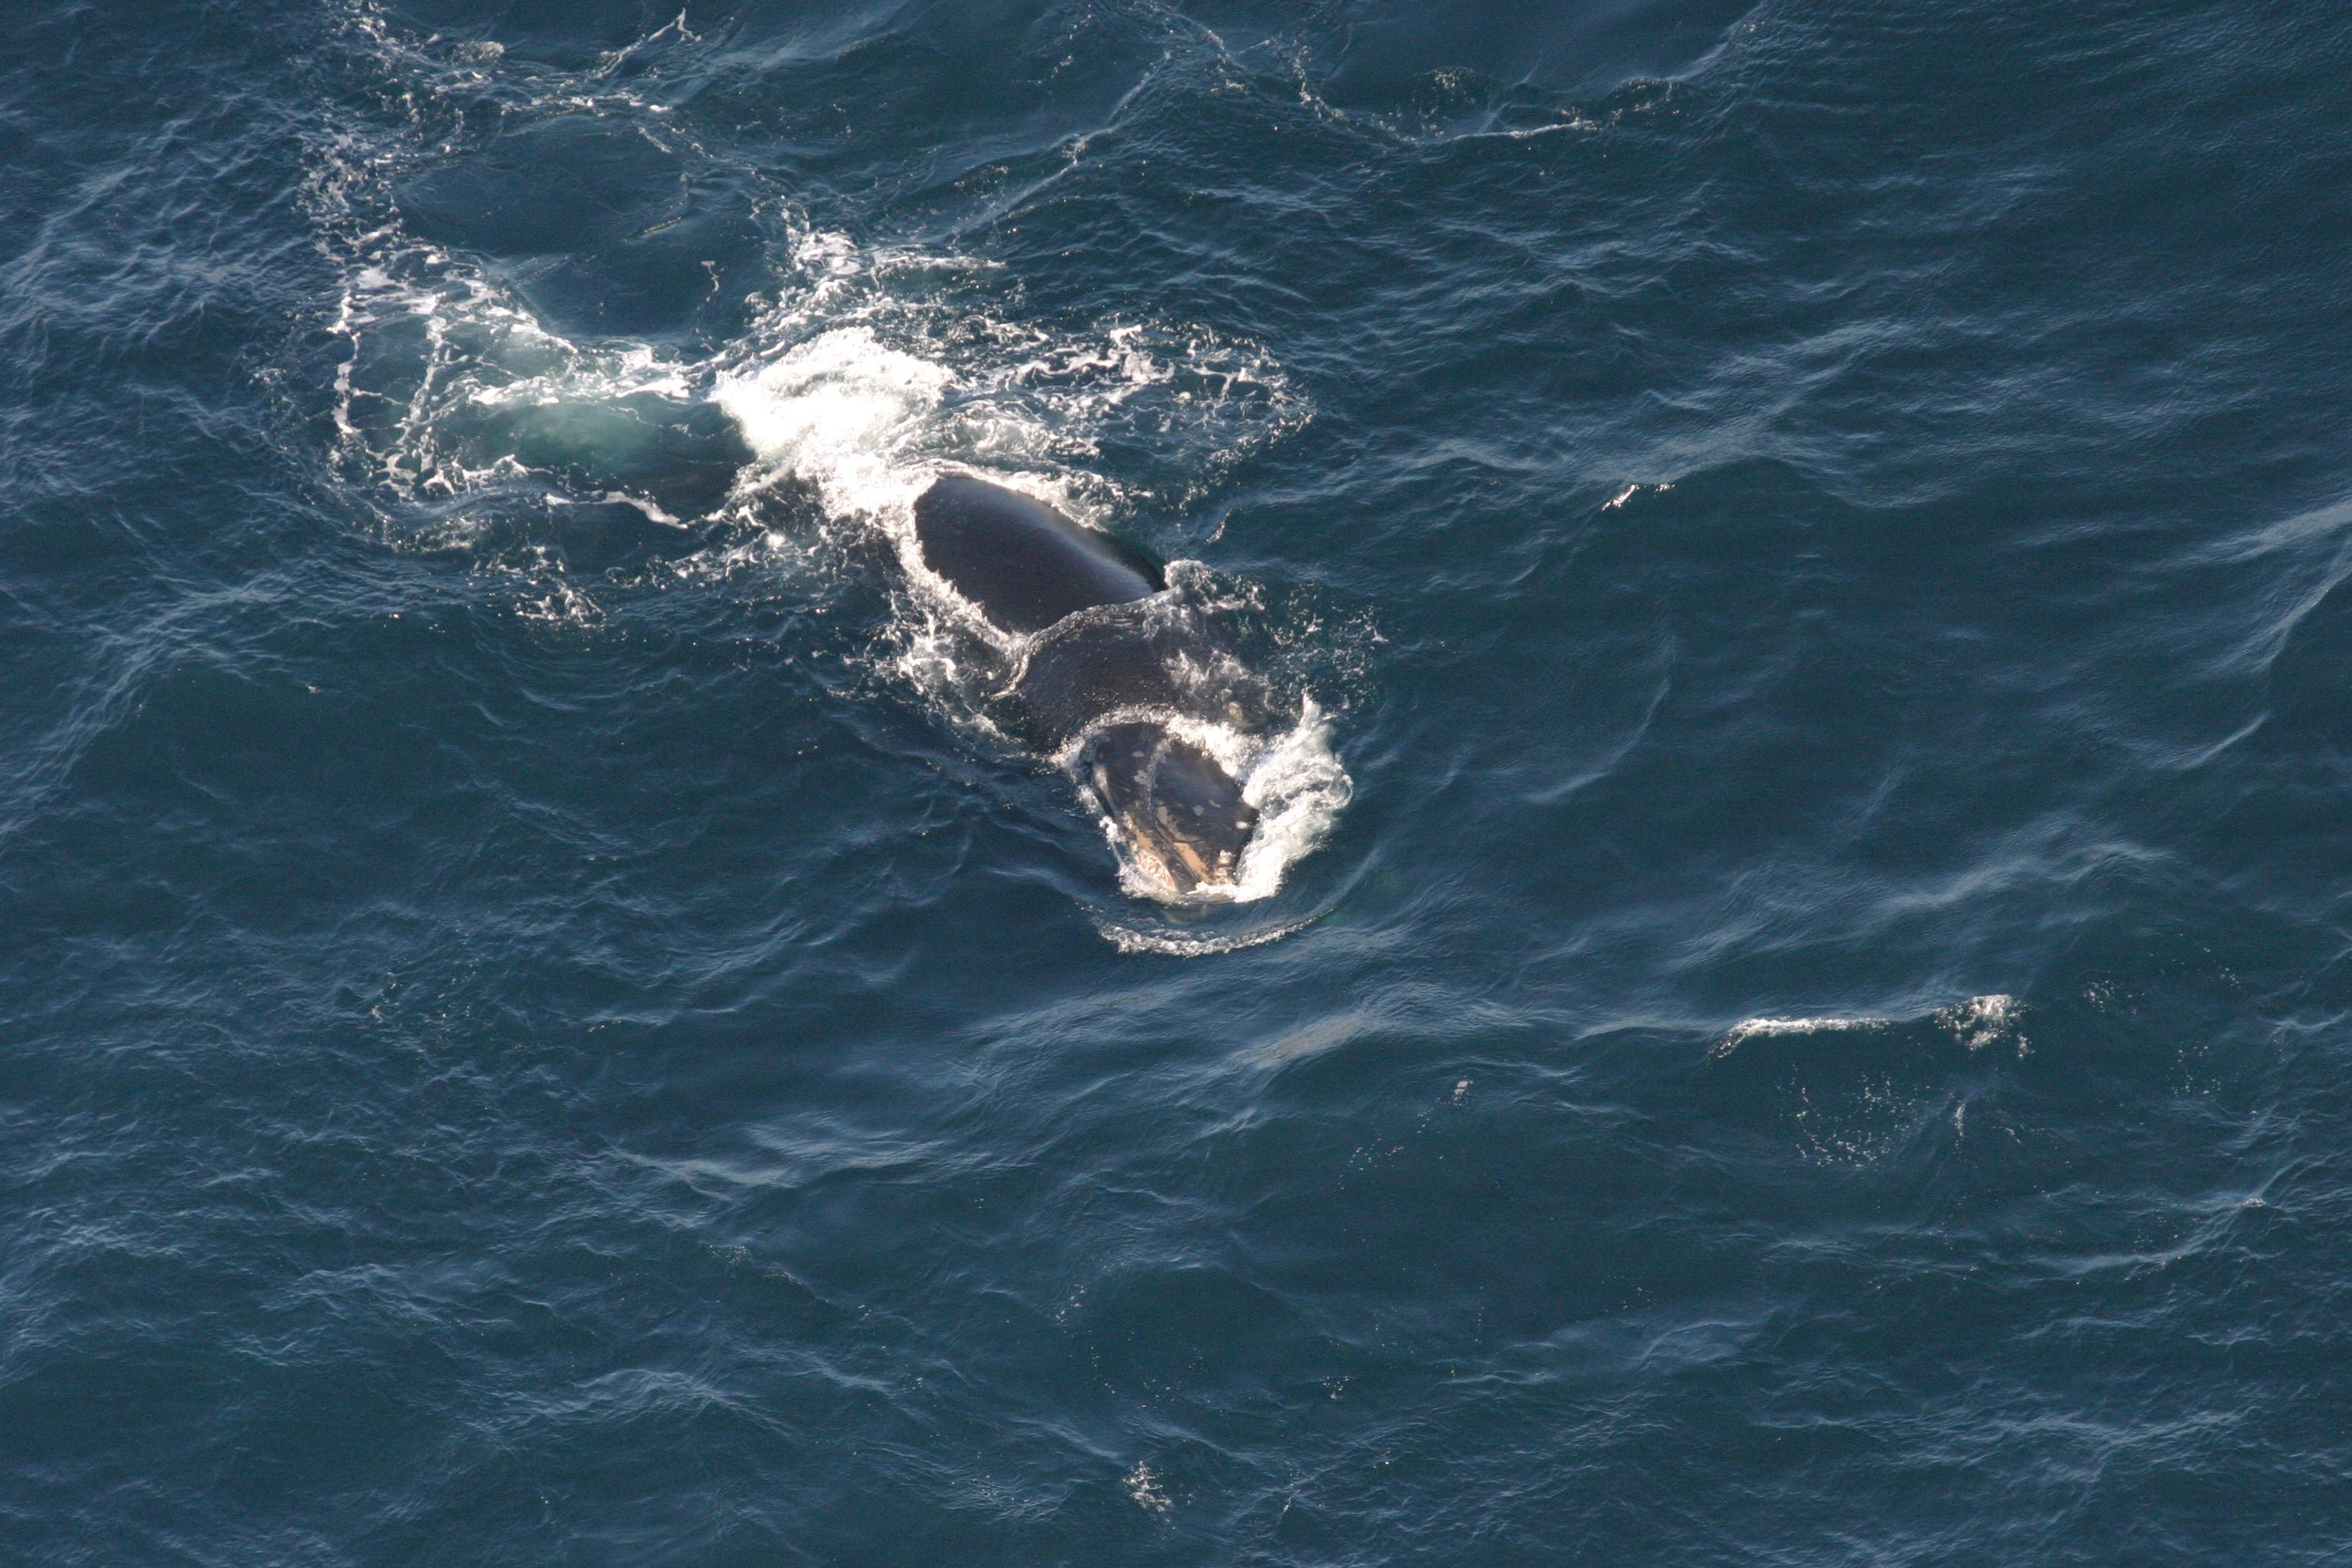
\includegraphics[scale=0.1]{foam.jpg}
	\centering
	\title{Example of a whale aerial picture with foam}
\end{figure}

\begin{figure}[H]
	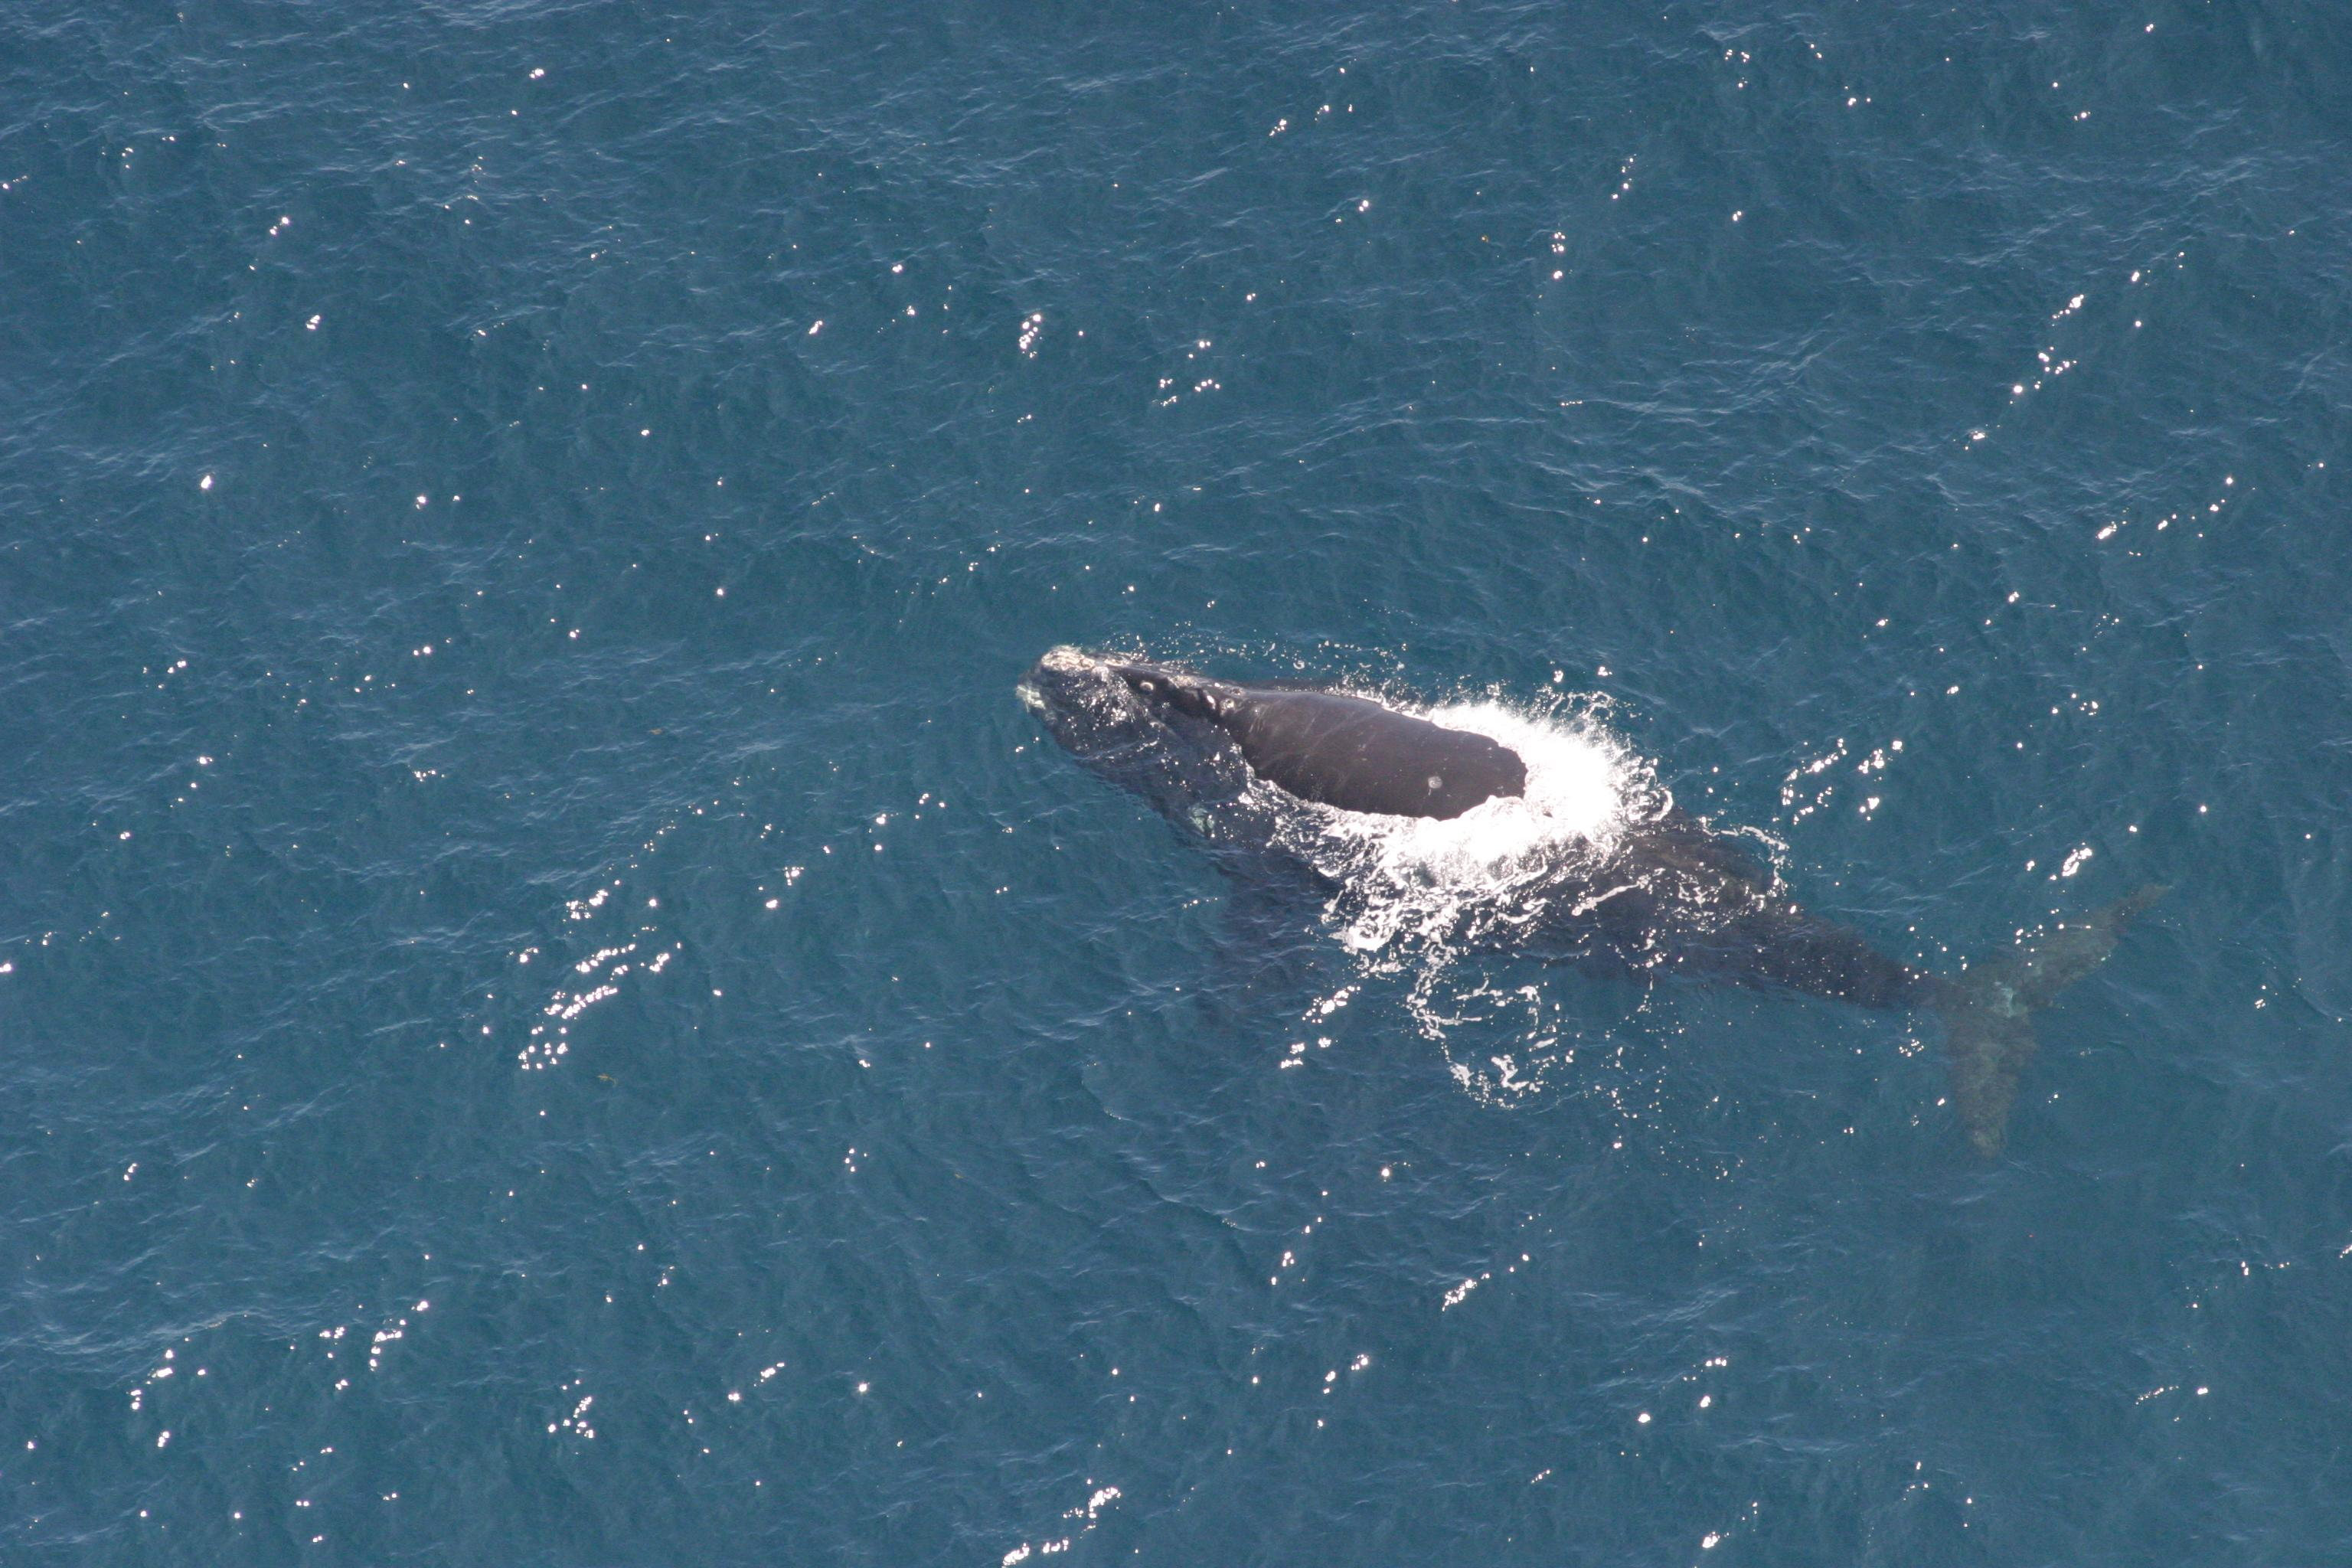
\includegraphics[scale=0.15]{water.jpg}
	\centering
	\title{Example of a whale aerial picture with shining water}
\end{figure}

\begin{figure}[H]
	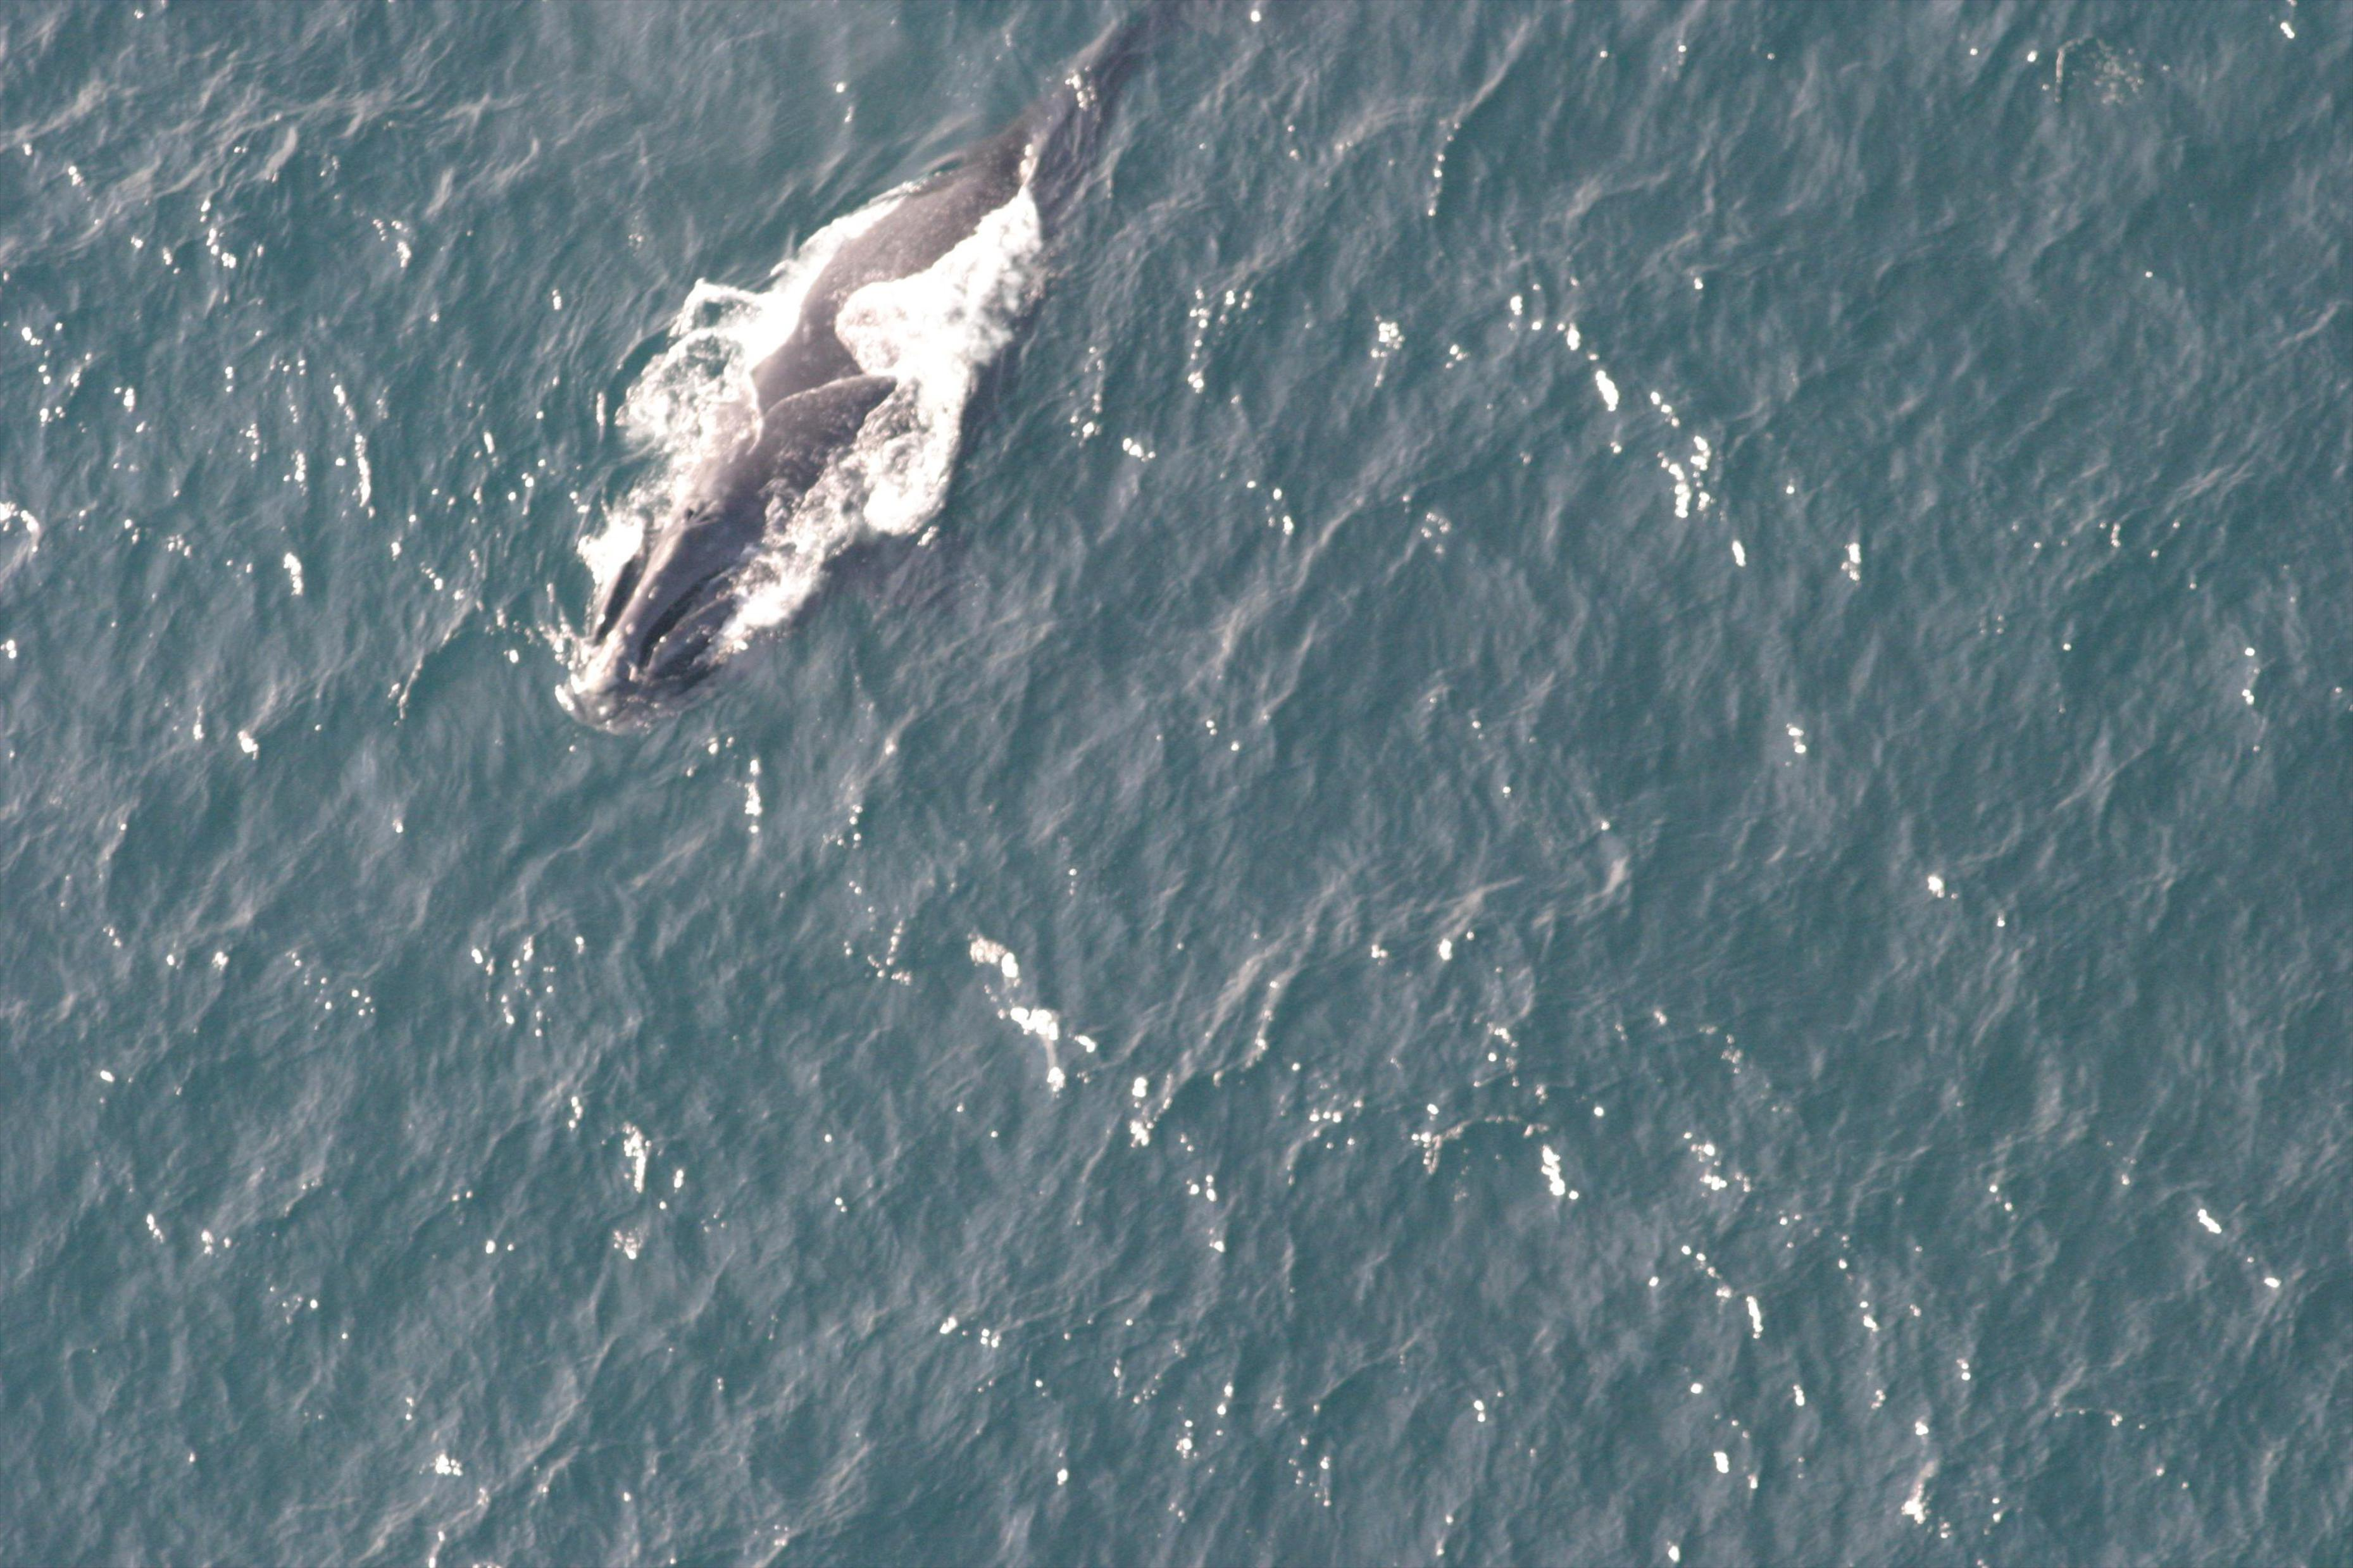
\includegraphics[scale=0.1]{invisible.jpg}
	\centering
	\title{Example of a whale aerial picture where the callosities are not visible}
\end{figure}

\begin{figure}[H]
	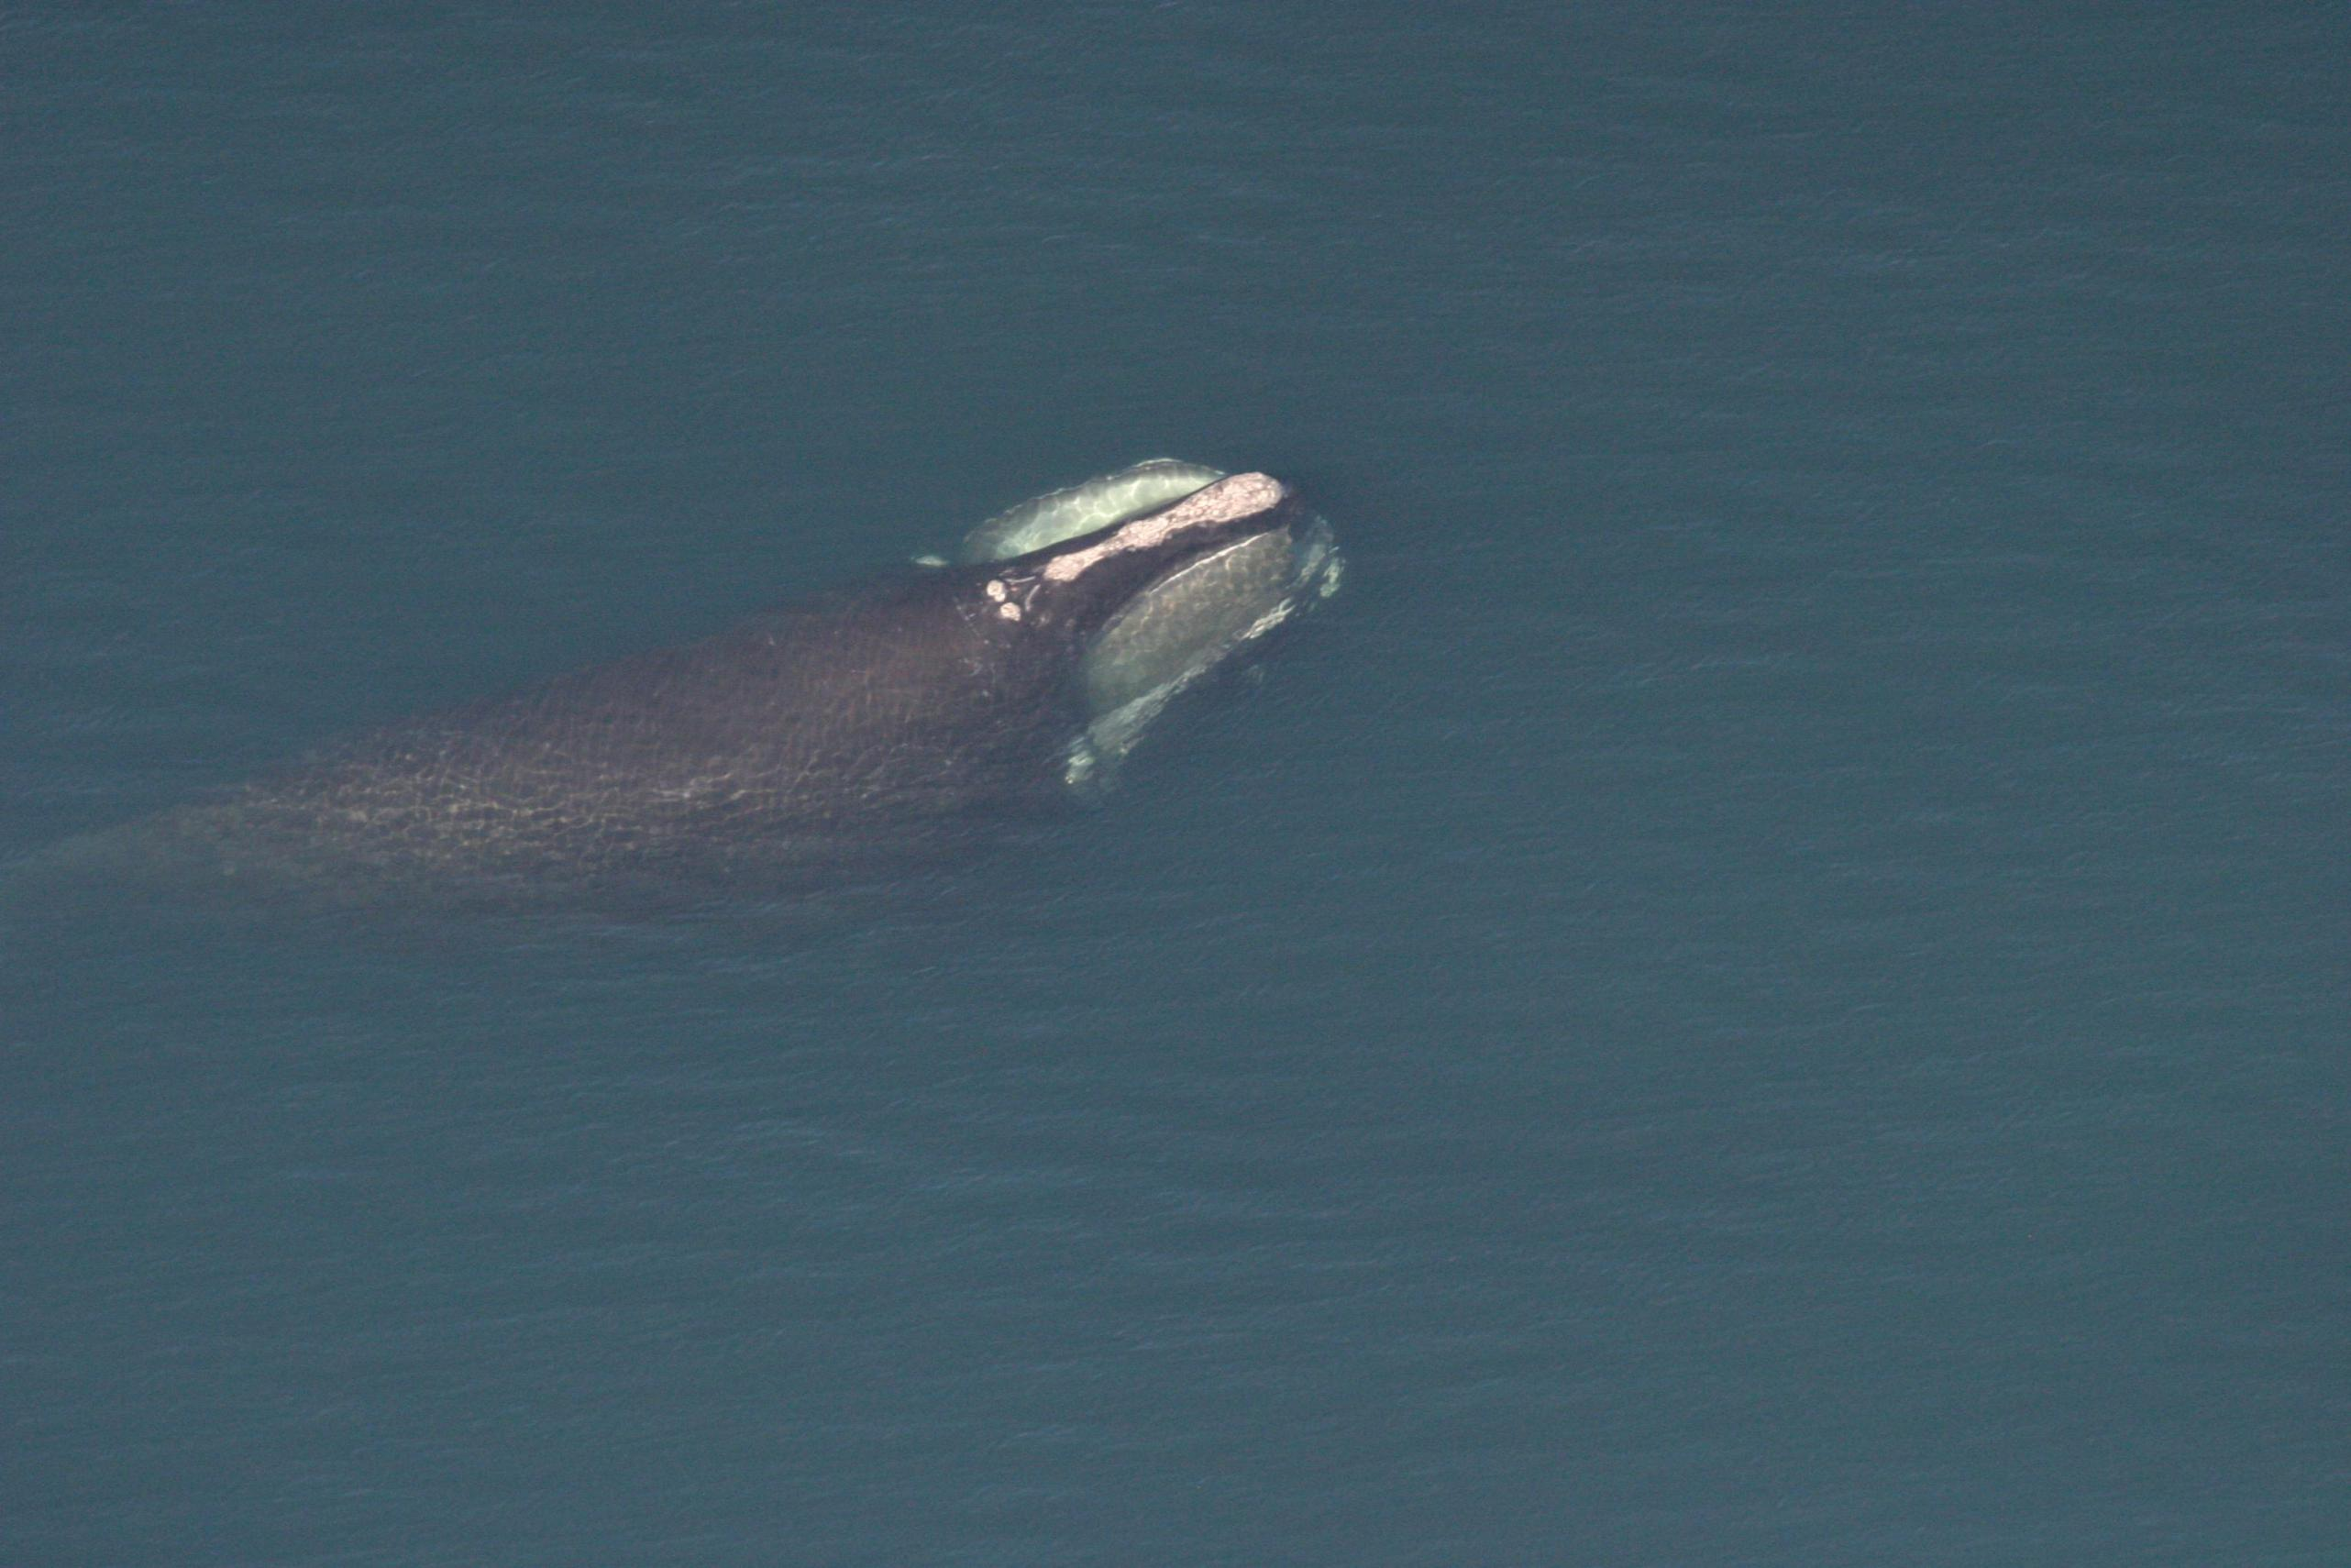
\includegraphics[scale=0.15]{better.jpg}
	\centering
	\title{Example of a relevant whale aerial picture}
\end{figure}

\end{appendices}

\end{document}
